\section{Future Work}
In the future we would like to attempt 3 things, the first being to train on even more games. There are approximately 4.5 trillion board states and we trained over at most 3.78 million. We believe that the filters may not have been fully trained resulting in worse performance. 

Another step we would like to try is to adjust the network structure. Currently we are passing the valid moves to the convolution layer. Convolving over the valid move information might hurt the networks ability to use this information. An alternative structure is shown in Figure~\ref{fig:struct_future}.

In this setup the valid moves information is directly fed into the final output layer. The idea here is that this would allow the final layer to quickly discard actions that would seem to have a $Q$-value but are actually invalid in the current state. 

A problem with the current network is that a large fraction of the initial negative reward it receives is due to it picking invalid actions. This may interfere with the goal to learn which of the \textit{valid} moves are best. Giving the final layer direct access to the valid moves information might result in the network learning to only pick valid moves faster. The network could then subsequently focus on learning which valid moves are most likely to result in a win.

Of course, this network structure and the one described earlier in this paper are only two possible solutions. Additional structures are certainly an option.

\begin{figure*}[t]
  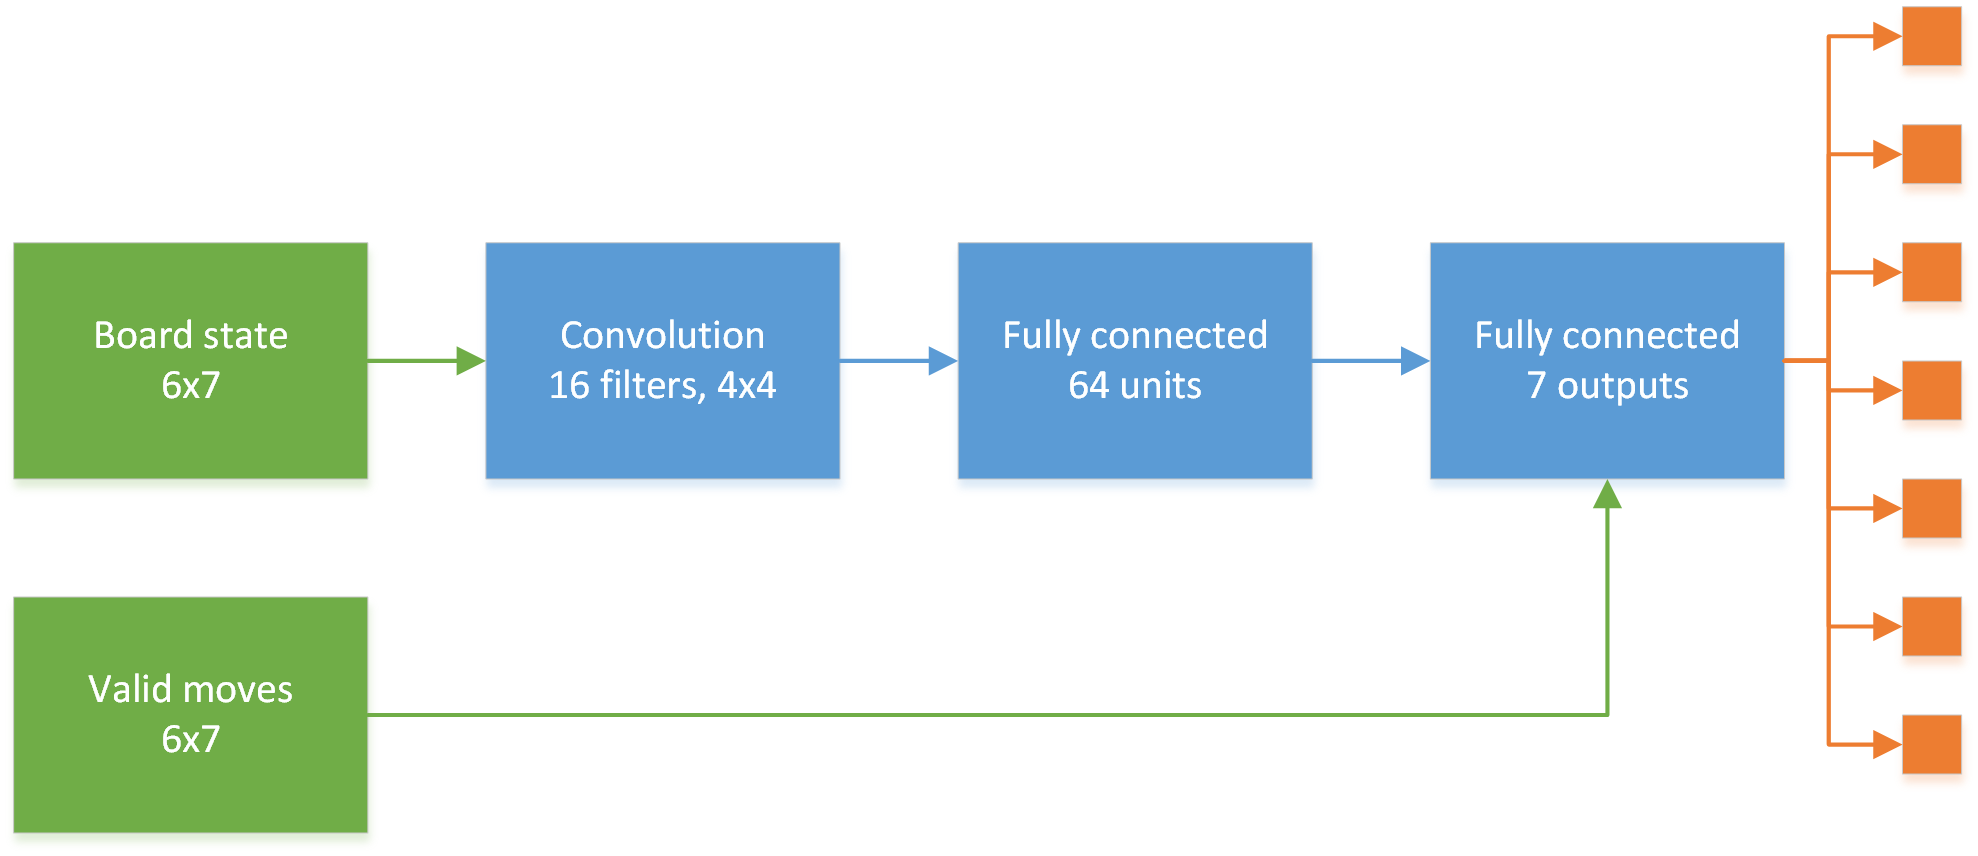
\includegraphics[width=\linewidth]{Network2.png}
  \caption{Possible future network structure}
  \label{fig:struct_future}
\end{figure*} 

Finally, we would like to attempt to incorporate memory. Just like a person will try to manipulate the game to get to a state where they know they can win, we would like to add that ability to the network. By giving a board state to the network which is close to our current board state and a state from which we have won before we could train the network to use the memory of past games to improve future games performance just like a person would do.